\documentclass[11pt,a4paper]{article}
\usepackage[utf8]{inputenc}
\usepackage[spanish]{babel}
\usepackage{amsmath}
\usepackage{amsfonts}
\usepackage{amssymb}
\usepackage{graphicx}
\usepackage{hyperref}
\hypersetup{%
  colorlinks=true,% hyperlinks will be coloured
  urlcolor=blue
}
\usepackage[left=2cm,right=2cm,top=2cm,bottom=2cm]{geometry}
\author{Diego Ramírez Milano \& Diego Zambrano Sierra}
\title{Proyecto Final Métodos Computacionales}
\date{Julio 21 de 2015}
\begin{document}
\maketitle
 
\section{\label{intro}Introdución}
{
El problema al cual decidimos acercarnos es el de los N-cuerpos. Esto entendido como un número finito de cuerpos distribuidos en el espacio los cuales interactúan debido a la fuerza de gravedad. Para solucionar el problema modelamos una simulación que toma las ecuaciones de movimiento de los cuerpos basados en la fórmula de gravitación universal propuesta por Newton y las resuelve de manera numérica utilizando el método Runge-Kutta de orden 4. En concordancia con lo anterior, además de realizar la simulación también se realiza una animación que permite apreciar de manera más sencilla el comportamiento de los cuerpos.\\

Ahora, para aplicar el código realizado a un supuesto de la vida real escogimos el sistema \textit{Gliese 667} para tomar de este sus datos e intentar reproducir su comportamiento. Todos los datos de dicho sistema se tomaron de de la base de datos \href{http://www.openexoplanetcatalogue.com/}{Open Exoplanet Catalog}. Así como de su versión en \href{https://github.com/OpenExoplanetCatalogue/open_exoplanet_catalogue}{Github} y los contenidos de \href{http://www.contact-conference.com/images/c12COTIsys.pdf}{este} documento.\\
}

\section{\label{marco}Marco Teórico}
{
La ecuación propuesta por Newton que describe la interacción gravitacional ejercida sobre una determinada masa por $N$ otras se presenta a continuación:
\begin{equation}\label{eq1}
m_i \frac{d^2 r}{dt^2} = -G \sum_{i \neq j} \frac{m_i m_j (r_i - r_j)}{|r_{i} - r_{j}|^3}
\end{equation}
donde $i,j = 1 \dots N$ y cada índice representa una masa particular, $r$ es el vector posición de cada masa y $G$ es la constante de gravitación universal ( $G = 6.67384 \times 10^{-11} \dfrac{m^3}{Kg\ s^2}$).\\

Para resolver estas ecuaciones de movimiento que surgen de cada masa a partir de la aplicación de la formulación de Newton utilizamos el método numérico de Runge-Kutta de orden 4. Este método toma una ecuación diferencial ordinaria de primer orden y por medio de aproximaciones numéricas arroja una solución de la ecuación diferencial. El método  exige que se tenga una ecuación de la siguiente forma:
\begin{equation}
\frac{d}{dt} Y(t) = f(Y)
\end{equation}
para nuestro caso si modificamos un poco la ecuación (\ref{eq1}) obtenemos
\begin{equation}
\frac{d}{dt}\left(\frac{d r}{dt}\right) = -G \sum_{i \neq j} \frac{m_j (r_i - r_j)}{|r_{i} - r_{j}|^3}
\end{equation}
ecuación que se acomoda al modelo de Runge-Kutta y por lo tanto puede ser aplicado a este supuesto para resolver las ecuaciones de movimiento y encontrar los valores de posiciones y velocidades de las masas luego de un tiempo de interactuar.\\

La ventaja de utilizar el cuarto orden del método Runge-Kutta es que es suficientemente complejo como para arrojar una solución moderadamente precisa y satisfactoria para realizar una simulación. Y a su vez no tan complejo como los órdenes superiores por lo que optimiza el tiempo de ejecución y procesamiento en el ordenador.
}

\section{\label{desa}Desarrollo}
{
Dado que la información en las bases de datos no se encuentran unidades estándar del sistema internacional se deben realizar ciertas modificaciones.\\
La unidad de \textbf{longitud} a utilizar es la unidad astronómica($UA$) la cual corresponde a $1.49598 \times 10^{11} m$.
La unidad de \textbf{masa} a utilizar son las masas de Júpiter($M_J$) la cual  corresponde a $1.898 \times 10^{27} Kg$.
La unidad de \textbf{tiempo} a utilizar son los días($d$) el cual corresponde a $86400 s$.\\

Realizando los cambios respectivos el nuevo valor de la constante de gravitación pasa a ser:
\begin{equation}
G = 2.824381 \times 10^{-7} \dfrac{UA^3}{M_J\ d^2}
\end{equation}
\subsection{\label{descr}Descripción del sistema}
{
Gliese 667 consta de dos estrellas(A y B) que forman un sistema binario al orbitar entre ellas al rededor de un centro imaginario. Están separadas por 13AU. Luego hay otra estrella (C) que también orbita al rededor de este centro imaginario peor dista de este 200AU. Asumiendo que A y B se encuentran sobre un mismo plano entonces C se encuentra a 50 grados de elevación.\\

A su vez, C forma un sistema ya que posee 7 planetas que lo orbitan. Se presume que también hay planetas orbitando a A y B pero dado que son tan pequeños no han podido ser medidos con exactitud y por lo tanto serán ignorados en este trabajo.
\begin{figure}[h!]
\begin{center}
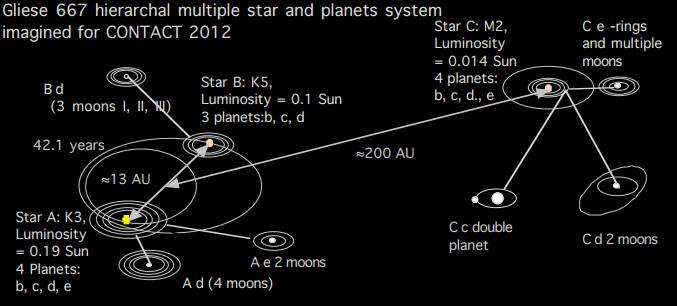
\includegraphics[scale=0.7]{G667.jpg}
\label{fig:G667}
\caption{Esquema de G667}
\end{center}
\end{figure}
}

Se tomará como origen virtual el punto sobre el cual las 3 estrellas orbitan. La información de las masas, velocidades y posiciones relativas iniciales de las cuales parte la simulación se pueden observar en este \href{https://github.com/diegolramirez/MC/blob/master/Proyecto/datos.csv}{.csv}.\\

El código donde está presente la solución al problema puede ser encontrado en el siguiente \href{https://github.com/diegolramirez/MC/blob/master/Proyecto/proyecto.ipynb}{cuaderno de ipynb}.
}
\end{document}